\documentclass[a4paper,12pt]{report}
\usepackage{graphicx}
\title{Report\\``MTSK-GAME''}

\author{Pietro Olivi\\
Leonardo Tassinari\\
Lorenzo Dalmonte\\
Alessio Paoloni}
\date{\today}


\begin{document}

\maketitle

\tableofcontents

\chapter{Analysis}
The software commissioned by the professors of the Object Oriented Pro\-gramming course aims to create an application designed to enhance psycho-motor skills through a gaming experience based on multitasking.\\
The term \textit{Multitasking} refers to the ability of a person or a product to do more than one thing at a time.

\section{Requirements}
\subsection*{Functional}
\begin{itemize}
	\item Upon starting, the software will display a simple minigame.\\
	A minigame is a potentially-never-ending challenge that requires simple actions from the player in order to keep the game going on.
	After a short amount of time a new minigame will appear and so on until all four minigames are shown.
	\item The player's goal is to surive as long as possible. After failing a minigame the application will display the final result, 
  therefore the software has to keep track of how long the player has lasted in the match in order to calculate the score.
\end{itemize}

\subsection*{Non functional}
\begin{itemize}
	\item The application shall sustain high framerate (around 120 fps) in all the sections of the gameplay, even on older hardware\footnote{e.g. Intel Core i3 (fourth generation), 4Gb of RAM.}.
	\item It shall be possible to easily develop and swap the minigames among the ones that best fit the training purposes of the user on top of those already provided. 
\end{itemize}



\section{Domain analysis}

MTSK-Game must exhibit some \textit{minigames}, the ones supplied by us are:
\begin{itemize} 
	\item \textit{WhacAMole} where the goal is to crush all the moles that emerge from the dug holes, before they re-enter them.
	\item \textit{DodgeATriangle} in which the player has to slide a \textit{rectangle} up and down switching lanes, aiming to avoid hitting moving \textit{triangles}.
	\item \textit{CatchTheSquare} where the user should collect \textit{squares} running over them with a \textit{circle} before they disappear.
	\item \textit{FlappyBirdAlike} where the user needs to control a \textit{cursor} leading it to fit between \textit{obstacles} that will come towards it.
\end{itemize}
For the game to end, and the \textit{score} to appear, it'll be sufficient losing in only one of the currently screened mingames.


\begin{figure}[h]
	\centering{}
	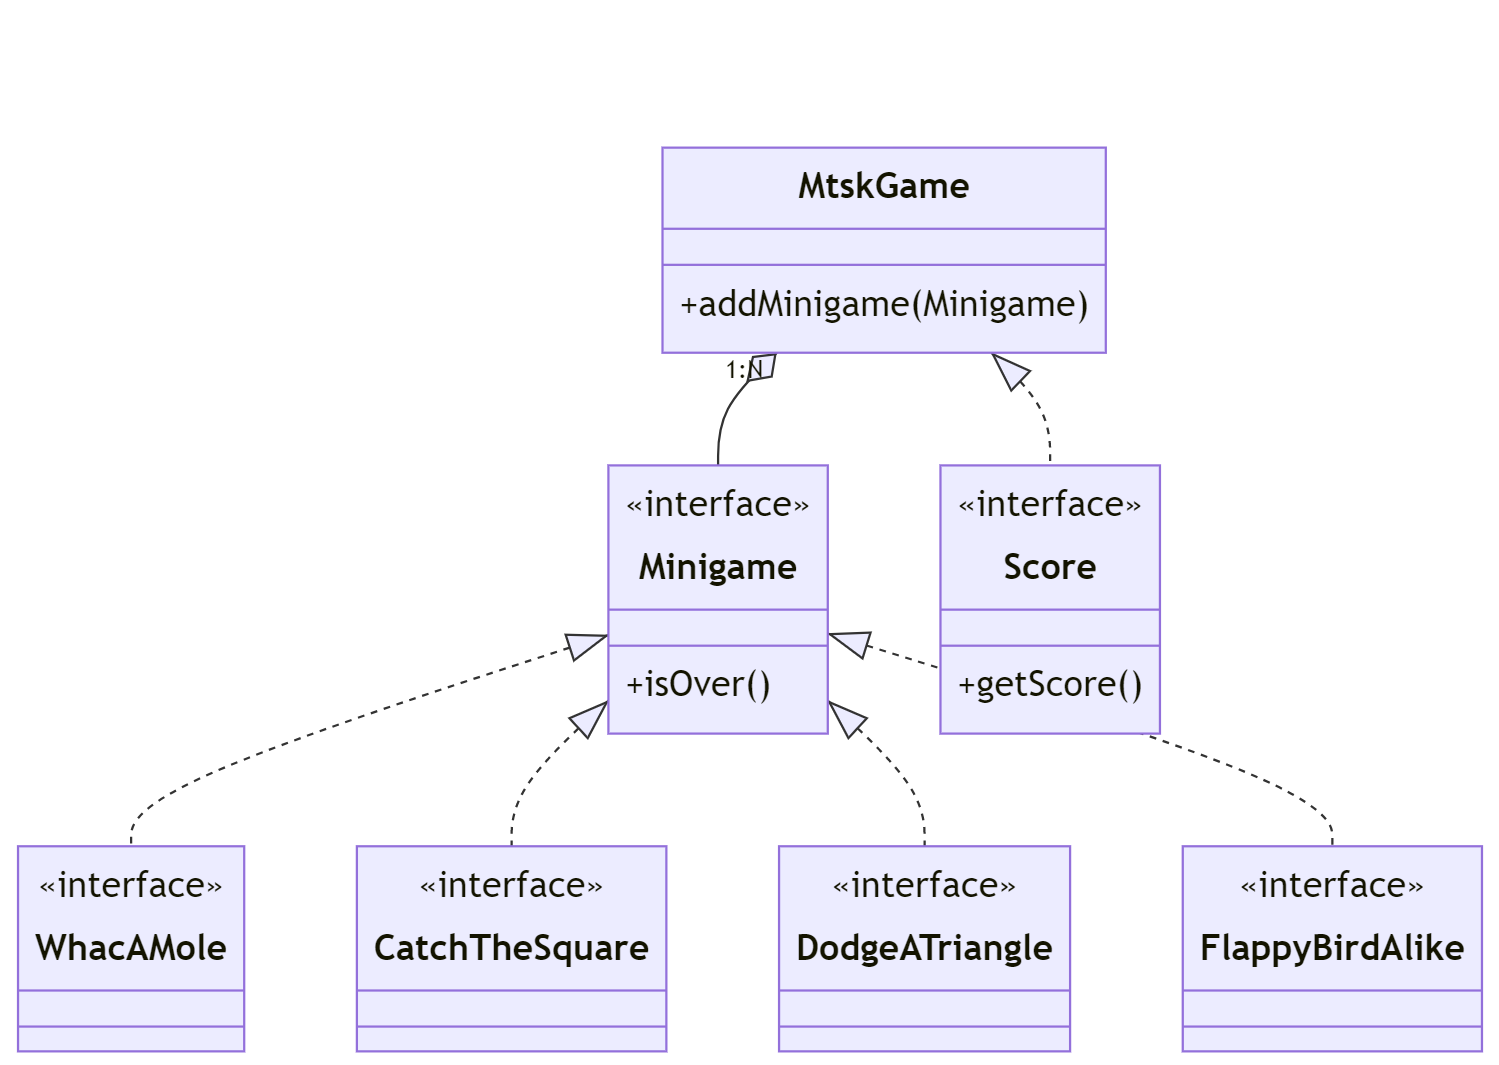
\includegraphics[width=\textwidth]{res/mermaid-diagram-2022-12-24-032504.png}
	\caption{UML diagram of the domain analysis}
\end{figure}

\chapter{Design}

\end{document}
